\addcontentsline{toc}{chapter}{Введение}
\chapter*{Введение}

Большое количество современных систем являются беспроводными. Простота развертывания, мобильность, относительно низкая
стоимость - вот основные преимущества беспроводных систем. Количество мобильных устройств (телефоны, планшетные компьютеры
и т.д.) с каждым годом стремительно растет, только мобильных телефонов в 2011 году было 5.6 миллиарда и покрывало 79.86\%
\cite{wiki_mobilenum} населения земли. Технологии беспроводной связи глубоко проникли во все сферы жизни общества:
обеспечение безопасности с помощью RFID датчиков, предоставление доступа в интернет по технологиями 3G, WiFi, 
сотовая связь по различным технологиям (GSM, CDMA, DAMPS). Некоторые из этих систем строятся на основе методики
расширения спектра, которая отвечает современным требованиям по мощности сигнала, а так же по безопасности передаваемых
данных. В основе таких систем лежат шумоподобные (широкополосные) сигналы - ШПС. Вместе с тем растут требования к таким
системам. Применение ШПС ставит ряд специфических задач по обработке информации, обусловленных особенностями ШПС.
Свойства характерные для ШПС, выгодно отличают данный класс систем от класса узкополосных систем, но с другой стороны
оборачивается усложнением методов обработки ШПС.

Внедрение новых технологий требует увеличение полосы частот. Разнообразие технологий беспроводной передачи данных среди
гражданских и военных систем ведет к перегрузке каналов связи и все более высоким требованиям к скорости передачи
данных. С учётом данных требований применение систем передачи информации с ШПС становится все более востребованным.

Принимая во внимание географические размеры России и стратегическую важность обладания собственными системами спутникового
позиционирования, правительство Российский Федерации уделяет особое внимание разработке собственной системы
глобального спутникового позиционирования ГЛОНАСС. Обладание собственными технологиями системы спутниковой навигации (СНС), государство может обезопасить
себя в случае военных конфликтов от ограничения применения американской системы СНС Navstar GPS в зоне конфликта.

Разработка систем, позволяющих работать с несколькими различными СНС, позволит повысить точность определения координат
в сложных условиях города. Сложность детектирования сигнала и определения координат обусловлена наличием плотной
застройки многоэтажными зданиями. В городских условиях задача подавления интерференционной помехи становится особенно
актуальной. Спектр интерференционной помехи не является белым, а фильтрация и компенсация цветного шума
требует разработки специальных алгоритмов.

Новые цифровые процессоры позволяют применять подходы, которые еще 10-15 лет назад были бесперспективными.
В данной работе развиваются подходы на основе построения параметрической модели ШПС. Невозможность использования
методов требующих вычислений с высокой точностью в приемниках реального времени
10-15 лет назад была обусловлена слабой производительностью процессоров и микроконтроллеров, а так же существенной
стоимостью процессоров с модулем для операций с числами с плавающей точкой. Современное развитие цифровых технологий делает 
возможным применение параметрических методов оценки спектра взамен традиционного подхода основанного на непараметрического
анализа спектра.

Основа теории систем связи с ШПС была заложена в работах В.А. Котельникова и К. Шеннона.
России в этой области занимаются В.И. Борисов, В.Б. Пестряков, В.И. Журавлев, М.И. Жодзишский, Б.И. Шахтарин, Л.Е.  Варакин, В.Е. Гантмахер и др.

Изначально методы расширенного спектра применялись при разработке военных систем управления и связи \cite{sklyar}.
К концу второй мировой войны расширение спектра применялось в радиолокации для борьбы с преднамеренными помехами, а
в последствии развитие данной технологии объяснялось желанием создать помехоустойчивые системы связи.
В конце 40-х-начале 50-х годов прошлого века Мортимер Рогофф, сотрудник Международной Телефонной и Телеграфной Корпорации (США) (ITT),
провёл эксперимент по передаче информации при помощи псевдошумового сигнала \cite{sklyar}, среди отечественных ученых
в середине 30-х годов прошлого века работу об основах кодового разделения каналов написал Д.В. Агеев.
Первые разработки таких систем относились к военным отраслям. Данный факт объясняется рядом особенностей, которыми обладают
сигналы с расширенным спектром, в числе которых — сложность перехвата заложенной в них информации,
высокая помехоустойчивость, а также трудность обнаружения факта работы передатчика. В процессе исследований расширенному спектру
нашлось и другое применение - снижение плотности энергии, высокоточная локация, использование при множественном доступе
\cite{sklyar}

Системы связи с широкополосными сигналами занимают особое место. Их особенные свойства выделяют данный класс из других систем
связи. Высокая помехозащищенность при действии сильной помехи, кодовое разделение большого количества абонентов, прием
информации с высокой достоверностью - отличительные особенности широкополосных система. Эти черты были известно, но
уровень элементной базы и низкий уровень помех не позволяли получить развития системам данного класса. Однако развитие
элементной привело к широкому распространению данного вида сигналов. В настоящее они применяются в системах спутниковой навигации,
системах сотовой связи и др \cite{varakin-book}.

Отношение сигнал/шум (ОСШ) на входе приемника может быть очень низким. Для обеспечения высокой помехозащищенности 
в таких случаях используются ШПС с большими и сверхбольшими базами.

К созданию сложных широкополосных сигналов (СШС) привело решение ряда проблем при развитии систем передачи данных.
Первая проблема встала при разработке новых радиолокационных система. Для дальнейшего развития требовалось
решить несколько противоречий: требование высокой разрешающей способности по дальности и дальностью обнаружения
целей в импульсных РЛС, требование точного измерения скорости и высокое разрешение по дальности, требование
увеличить дальность при ограничении пиковой мощности \cite{gantmaher-book}. Решение данных задач было предложено
Ф. Вудвардом. Им было показано, что дополнительным параметром является форма сигнала. Длительность сигнала
может быть больше - настолько больше, насколько это необходимо для обеспечения энергетических требований, а требование
разрешения по дальности и точности измерений определяются шириной полосы сигнала. Данные требования обеспечивается
путем сжатия импульса на стороне приемника. Вудворд сформулировал принципы: произведение эффективной полосы частот
радиосигнала на его длительность должен быть существенно больше единиц ${FT>>1}$, внутренняя структура сигнала
должна быть такой, чтобы обеспечить возможность приемнику сжатие распределенного во времени сигнала в короткий импульс,
соответствующий полосе ${F}$ \cite{gantmaher-book}.

В \cite{gantmaher-book} показана связь пропускной способности канала с понятием ШПС. При ${R_e<<1}$ можно записать:
\begin{equation}
	%\label{eq:shennon_cdma}
	FT = \frac{1}{\log(1+R_e)}, \nonumber
\end{equation}
где ${R_e}$ - ОСШ, ${F}$ - эффективная полоса частот, ${T}$ - длительность.

Стоить отметить, что при ${R_e<<1}$, левая часть данного выражения стремится к бесконечности, а значит
ШПС позволяет обеспечить теоретически неограниченную достоверность передачи информации. Второе важное свойство
ШПС - способность работать "под шумами". Что обеспечивает скрытность
передачи информации, а с другой высокую степень уплотнения каналов связи и, как следствие, решение современных проблем
с перегруженностью каналов связи.

В данной работе будет рассматриваться ШПС модулированный ПСП на основе двоичной рекуррентной последовательности.
Для выделения данных из потока необходимо иметь точно синхронизированную копию ПСП, которая была использована
при модулировании сигнала на передающей стороне. Для достижения синхронизма на стороне приемника необходимо
устранить неопределенность в двух областях: неопределенность по частоте и неопределенность по фазе (задержке) ПСП.
Неопределенность по фазе ПСП обусловлена неопределенностью в расстоянии между передатчиком и приемником. Неопределенность
по частоте обусловлена в первую очередь допплеровским эффектом, а так же нестабильностью опорных генераторов в
передатчике и приемнике. После устранения неопределенности по частоте для достижения точной синхронизации
начинается процесс слежения за частотой. Неопределенность по фазе ПСП устранить, не используя полный перебор,
невозможно в силу корреляционных свойств ПСП. Таким образом можно заключить, что задача быстрого и эффективного
поиска и оценки параметров ШПС является актуальной.

В данной работе рассматривается подход программного приемника (Software Defined Receiver - SDR)
\cite{akos-book, grayver-book, pany-book} для оценки параметров ШПС. Как уже было отражено выше, ШПС применяется во
многих системах. В данной работе для полунатурного эксперимента будет рассматриваться сигнал СНС Navstar GPS. Данная система передачи 
информации (СПИ) использует ПСП Голда \cite{gold-ieee} для модулирования сигнала.

Традиционные подходы к реализации приемника СНС Navstar GPS отражены в \cite{akos-book, tsui}. 

Популярность и распространенность данной системы стимулирует исследования в области детектирования
и оценки параметров ШПС сигнала.

Существуют исследования в области применения теории хаоса - детектирование и оценка
частоты ШПС с применением осциллятора Дуффинга \cite{chaos_cambridge, chaos_chen, chaos_huang, chaos_wang}. Преимуществом
данного подхода является то, что свойства осциллятора позволяют детектировать сигналы с экстремально низким ОСШ.

Осциллятор Дуффинга с гармоническим внешним воздействием может быть описан уравнением:
\begin{equation}
	\label{eq:duffing}
	mx'' + cx' + k_{1}x + k_{2}x^3 = F_{0}\cos(\omega{t}),
\end{equation}
где $m$ - масса, $c$ - коэффициент диссипации, $x$ - состояние осциллятора, $k_1$ и $k_2$ - линейный и нелинейный коэффициенты соответственно,
$F_{0}\cos(\omega{t})$ - внешнее воздействие.

Подробно уравнение \ref{eq:duffing} рассмотрено в \cite{chaos_neimark_landa}.
Для использования осциллятора Дуффинга с целью оценки параметров ШПС была предложена усовершенствованная форма \cite{chaos_song, chaos_chen}:
\begin{equation}
	\label{eq:duffing_gps}
	x'' +cx' - x^3 + x^5 = \gamma\cos(\omega{t}) + (\gamma_{x}\cos(\omega_{x}) + n(t))
\end{equation}

Можно переписать динамическую систему \ref{eq:duffing_gps} в виде:
\begin{equation}
	\label{eq:duffing_gps_2}
	\left\{
	\begin{aligned}
		y(t) & = x'(t) \\
		y'(t) & =  -cx' + x^3 - x^5 + \gamma\cos(\omega{t}) + (\gamma_{x}\cos(\omega_{x}) + n(t)),
	\end{aligned}
	\right.
\end{equation}
где ${n(t)}$ - аддитивный Гауссовский белый шум (АБГШ), имеющий нулевое среднее  значение и КФ ${R_n(\tau) = \frac{N_0}{2} \delta(\tau)}$,
а ${N_0}$ - односторонний энергетический спектр.

Пример фазового портрета при ${\omega=\omega_{x}}$ изображен на Рис. \ref{pic:duffing_sync},
фазовый портрет хаоса расположен на Рис. \ref{pic:duffing_chaos1}, Рис. \ref{pic:duffing_chaos2}
\begin{figure}[h]
	\center\scalebox{0.5}{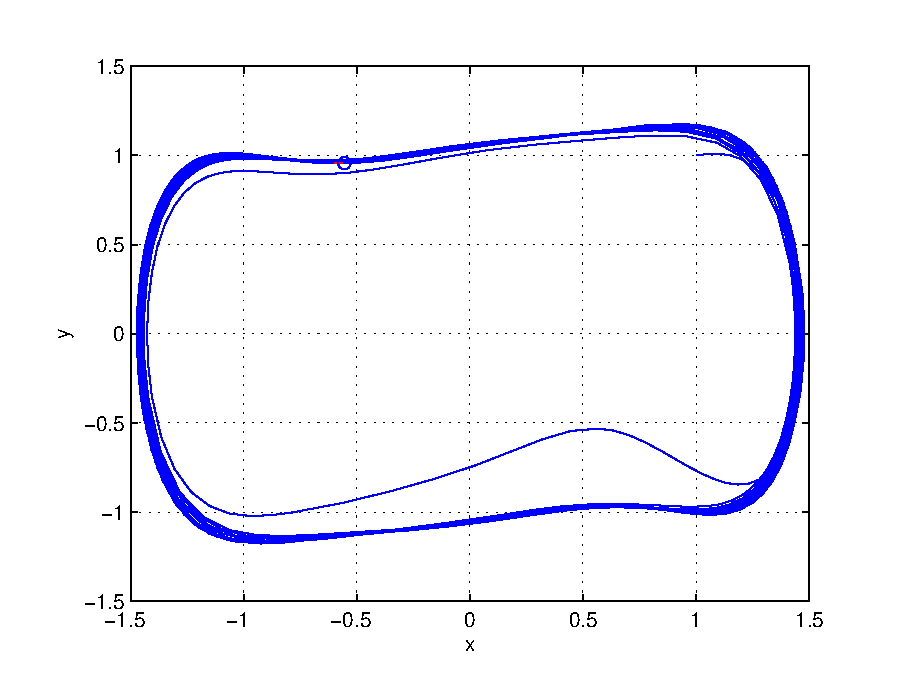
\includegraphics[width=1\linewidth]{duffing_sync.eps}}
	\caption{Фазовый портрет при ${\omega =\omega_{x}}$}
	\label{pic:duffing_sync}
\end{figure}
\begin{figure}[h]
	\center\scalebox{0.5}{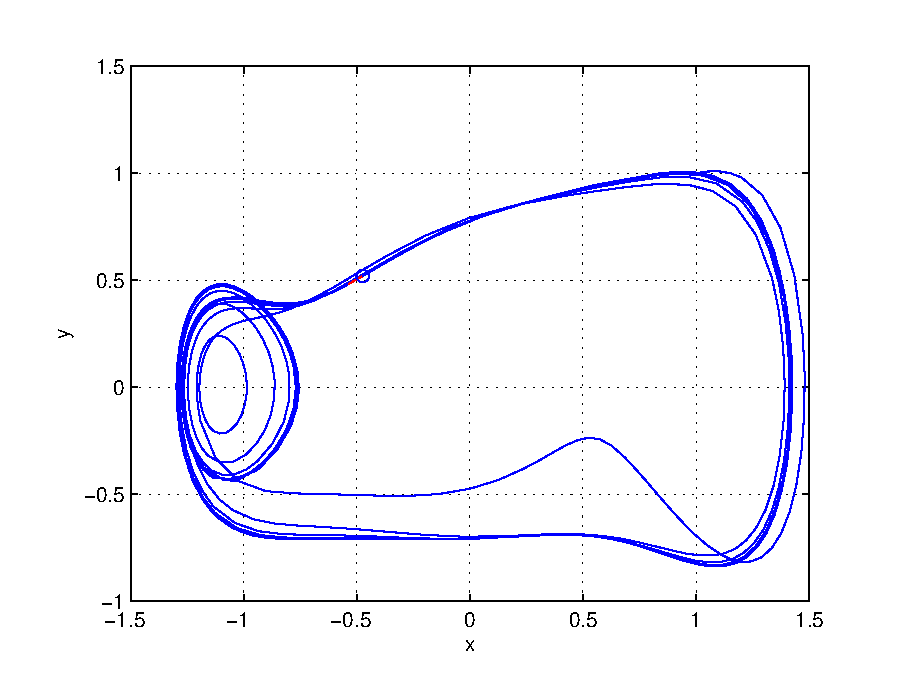
\includegraphics[width=1\linewidth]{duffing_chaos1.eps}}
	\caption{Фазовый портрет при ${\omega < \omega_{x}}$}
	\label{pic:duffing_chaos1}
\end{figure}
\begin{figure}[h]
	\center\scalebox{0.5}{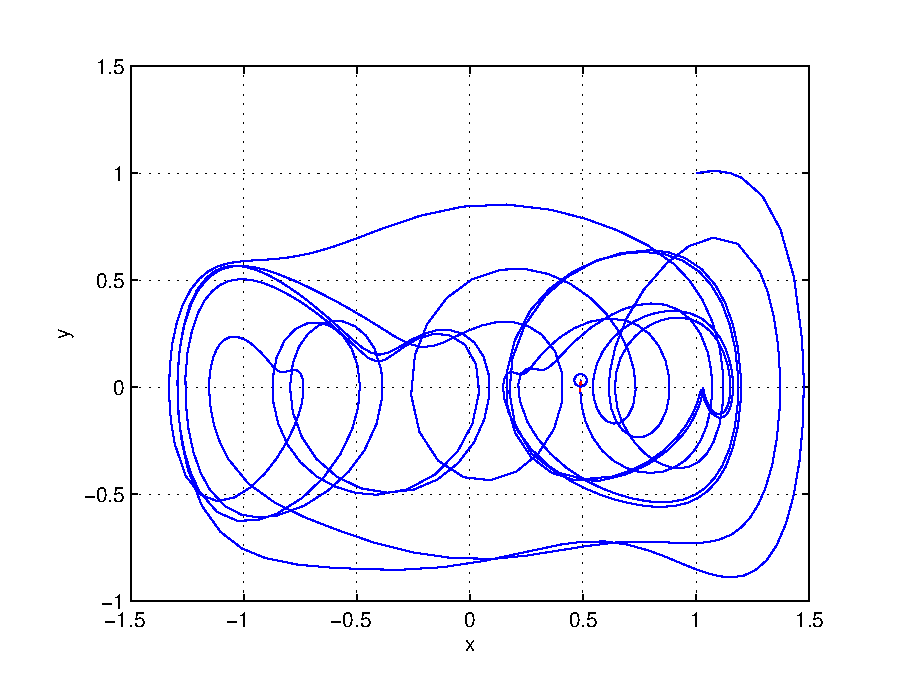
\includegraphics[width=1\linewidth]{duffing_chaos2.eps}}
	\caption{Фазовый портрет при ${\omega > \omega_{x}}$}
	\label{pic:duffing_chaos2}
\end{figure}
В качестве параметров уравнения применялись: $c = 0.5$, $\gamma=\gamma_{x}=0.36$, ${\omega=1}$

Часто для вычисления характеристик хаотической динамики применяется показатель Ляпунова.
Он показывает в каком состоянии находится система. Если система находится
в стабильном состоянии линии фазовой траектории будут близко прилегать одна к другой, в противном
случае система находится в состоянии хаоса. Детектор с применением показателя Ляпунова
представлен на Рис. \ref{pic:chaos_lyapunov}.
\begin{figure}[h]
	\center\scalebox{0.7}{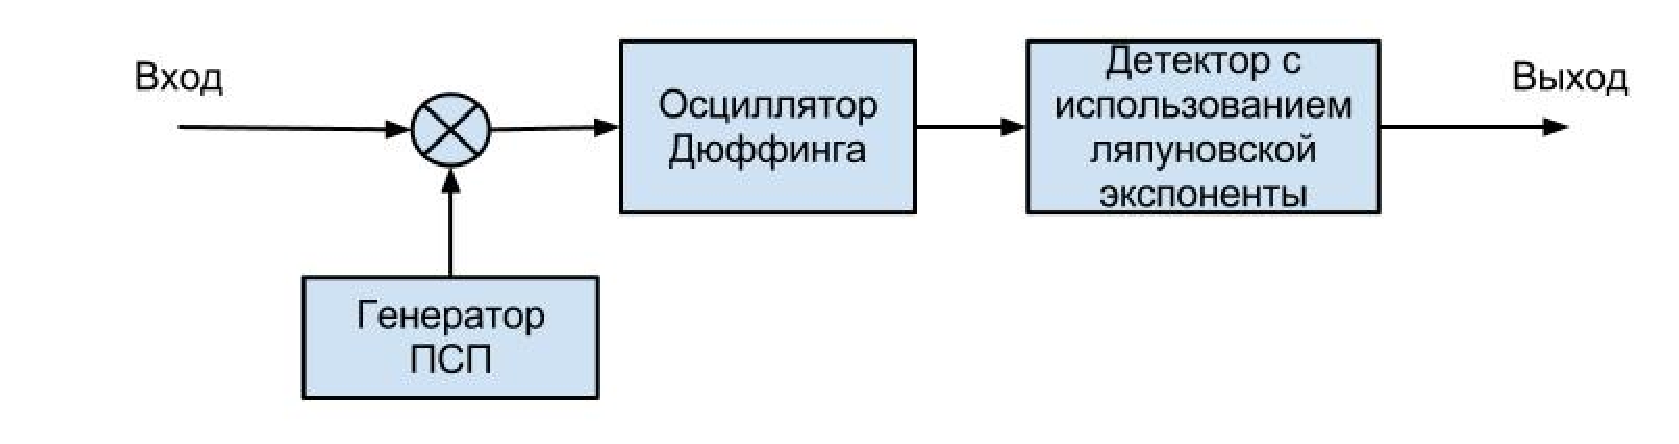
\includegraphics[width=1\linewidth]{Chaos_detector_Lyapunov.eps}}
	\caption{Схема детектора основанного на показателе ляпунова для осциллятора Дуффинга}
	\label{pic:chaos_lyapunov}
\end{figure}

В статье \cite{chaos_chen} предложен усовершенствованный метод, базирующийся на вычислении дисперсии
фазовой траектории. Действительно, на Рис. \ref{pic:duffing_sync}, \ref{pic:duffing_chaos1} и
\ref{pic:duffing_chaos2} видно, что когда система находится в хаотическом состоянии значение
дисперсии по координате ${x}$ больше, чем соответствующее значение в состоянии $\omega = \omega_{x}$.
На основе этого была предложена усовершенствованная схема детектора сигнала - Рис. \ref{pic:chaos_energy_detector}
\begin{figure}[h]
	\center\scalebox{0.7}{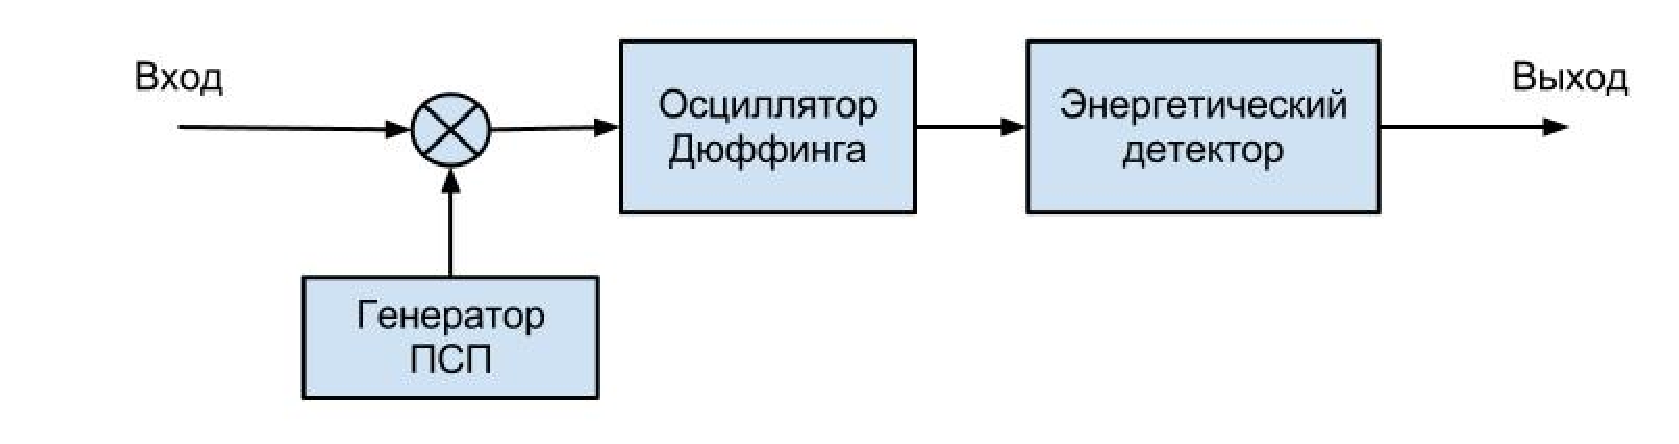
\includegraphics[width=1\linewidth]{chaos_detector.eps}}
	\caption{Схема энергетического детектора для осциллятора Дуффинга}
	\label{pic:chaos_energy_detector}
\end{figure}

В то же время, на данный момент никто не предложил цифровое представление осциллятора Дуффинга, а это затрудняет использование данного подхода
в реальных приемниках. Таким образом данное направление является в настоящее время больше теоретическим, чем практическим.

В работах \cite{hos_petropulu, hos_zhao} предложено использовать статистики высоких порядков для подавления шума и оценки
сигналов с низким уровнем ОСШ.

Интересная группа алгоритмов основывается на информационной избыточности ШПС, например \cite{phd_che}. В данной
группе алгоритмов используется механизм появления нескольких точек на основном пике КФ, описанный в \cite{kaplan}. Пример
изображен на Рис. \ref{pic:sec1_peak_tcd}.
\begin{figure}[h]
	\center\scalebox{1}{\includegraphics[width=1\linewidth]{corr_peak_tcd.eps}}
	\caption{Идеальная КФ ШПС с отмеченными точками возможного обнаружения}
	\label{pic:sec1_peak_tcd}
\end{figure}

На Рис. \ref{pic:sec1_peak_tcd} изображен пик КФ с несколькими точками. Две точки находятся выше порога ${\Pi=0.5}$.

В работе \cite{phd_che} рассмотрено создание субоптимального обнаружителя на основе информационной избыточности ШПС.
Получена целевая для системы синхронизации в целом и намечены дальнейшие пути развития данного направления.

Математический аппарат статистик высоких порядков (СВП или HOS - Higher-order statistics)
для исследования непричинных, причинных и нестабильных
(систем с неминимальной фазой) и не-Гауссовых сигналов впервые был предложен в \cite{hos_petropulu} в 1993 году.
Этот метод позволяет не только подавлять цветной Гауссов шум, но так же в некоторых случаях подавлять
цветной не-Гауссов шум. В работе \cite{hos_zhao} был предложен метод оценки параметров ШПС с использованием СВП.

Более традиционные подходы оценке параметров ШПС сигналов с низким уровнем ОСШ рассмотрены в монографии \cite{ziedan-book}.
В данной монографии рассматриваются как методы детектирования и оценки параметров ШПС, основанные на когерентном накоплении, так и эффективные
системы слежения за частотой и фазой ПСП.

Так же публикуются работы по выбору порога в алгоритмах захвата ШПС. Например в работах \cite{2max_ieee, 2max_article} представлен алгоритм
\textquotedblleft{Peak-finding algorithm}\textquotedblright,
в данной работе введем перевод -
\textquotedblleft{Алгоритм нахождения пика}\textquotedblright (АНП). 

Предложенный в работах алгоритм можно разбить на несколько шагов:
\begin{itemize}
	\item[Шаг 1] Подсчитать КФ, используя БПФ.
	\item[Шаг 2] Найти главный пик КФ, найти второй пик КФ, найти среднее значение КФ.
	\item[Шаг 3] Нормализовать полученные значения относительно главного пика КФ.
	\item[Шаг 4] Если (максимум КФ - среднее) > ${\Pi_1}$ и (максимум КФ - 
		второй максимум КФ) > ${\Pi_2}$, тогда принимается решение о наличии сигнала в принимаемой смеси. 
\end{itemize}

В статье авторов \cite{2max_ieee} предложены следующие значения для порогов:
${\Pi_1} = 0.3$ дБ и  ${\Pi_2} = 0.15$ дБ. Так же авторы предлагают итерационную процедуру для нахождения фазы ПСП и частоты смещения Допплера:
\begin{itemize}
	\item[Шаг 1] Начать вычисление с 1 мс.
	\item[Шаг 2] Получить результаты АНП.
	\item[Шаг 3] Если фаза ПСП и частота не могут быть найдены, увеличить время интегрироавния сигнала.
		Использовать следующие значения для интегрирования: 1мс -> 10мс -> 50мс -> 100мс -> 200мс -> 500мс -> 1000мс
\end{itemize}

%%%%%%%%
{\bf{Цель и задачи диссертации}}

Целью диссертационной работы является разработка и анализ алгоритмов оценки информационных параметров сигнала в системах с кодовым разделением каналов на основе
параметрического метода оценки частоты на фоне аддитивного белого гауссового шума и интерференционной помехи,
с возможностью реализации на современной элементной базе.

Для достижения поставленной цели в диссертации решаются следующие задачи:
\begin{enumerate}
	\item {С использованием методов параметрической идентификации автором разработан алгоритм оценки информационных параметров для одного источника сигнала
		в CDMA-системах на фоне аддитивного белого гауссового шума.}
	\item {Адаптация алгоритма повышения отношения сигнал/шум при оценке автокорреляционной функции гармонического сигнала для использования при обработке
		CDMA-сигнала в приемниках реального времени.}
	\item {Разработка комплексированного алгоритма оценки информационных параметров CDMA-сигнала на фоне аддитивного белого гауссового шума и
		интерференционной помехи, основанный на алгоритме Delay and Multiply Approach, алгоритме повышения сигнал/шум в оценке автокорреляционной функции 
		и авторегрессионной модели второго порядка.}
	\item {Сравнительный анализ разработанных алгоритмов с типовыми решениями в области оценки информационных параметров сигнала используемых в CDMA-системах.}
	\item {Полунатурное моделирование с использованием аппаратной платформы на реальных данных CDMA-системы Navstar GPS.}
\end{enumerate}

{\bf{Научная новизна результатов}}
\begin{enumerate}
	\item{На основе теории параметрической идентификации автором разработан алгоритм оценки информационных параметров сигнала в системах с кодовым разделением каналов.}
	\item{Предложен алгоритм компенсации окрашенного шума на основе итеративного вычисления автокорреляционной функции для
		получения несмещенной оценки частоты с использованием параметрического метода оценки спектра.}
	\item{Предложен способ эффективного итеративного вычисления автокорреляционной функции в базисе Фурье для использования в
		приемниках реального времени.}
	\item{Предложен способ комплексирования алгоритмов оценки фазы псевдослучайной последовательности (ПСП) Delay And Multiply Approach, алгоритма итеративной оценки АКФ и
		параметрического метода оценки спектра в задаче оценки параметров сигнала с расширенным спектром.}
\end{enumerate}

{\bf{Практическая ценность}}
\begin{enumerate}
	\item {Усовершенствован алгоритм повышения отношения сигнал/шум при оценке автокорреляционной функции. Оптимизация вычислительных затрат позволяет использовать
		данный алгоритм в приемниках реального времени.}
	\item {Комплексированный алгоритм оценки информационных параметров CDMA-сигнала позволяет существенно снизить вычислительные затраты.}
	\item {Программно-аппаратный стенд для экспериментального исследования систем цифровой связи с использованием технологии CDMA,
		позволяет подтвердить схемотехническую реализуемость разработанных алгоритмов.}
\end{enumerate}

{\bf{Апробация результатов}}

Результаты диссертации прошли аппробацию на:
\begin{enumerate}
	\item 7-ой Всероссийской конференции «Радиолокация и радиосвязь» (Москва 2013 г.);
	\item Международной конференции «Радиоэлектронные устройства и системы для инфокоммуникационных технологий - РЕС-2013» (Москва 2013 г.);
	\item V Международной студенческой научно-практической конференции «Интеллектуальный потенциал XXI века: ступени познания» (Новосибириск 2011 г.).
\end{enumerate}

{\bf{Внедрение результатов работы:}}
\begin{enumerate}
	\item Результаты диссертации использованы в НИОКР ЗАО «Теллум», что подтверждено актом о внедрении.
	\item Результаты диссертации использованы в учебном процессе на кафедрах автономных информационных и управляющих систем МГТУ им. Н.Э. Баумана,
		что подтверждено актом об использовании и управление и моделирование систем Московского Государственного Университета Приборостроения
		и Информатики, что подтверждено актом об использовании.
\end{enumerate}

{\bf{Объем и структура диссертации}}

Диссертация состоит из введения, четырех глав, заключения и списка литературы. Общий объем составляет XXX страниц, включающих XX страниц приложения, XX иллюстраций,
X таблицы и список литературы из XX наименований.

{\bf{Положения, выносимые на защиту}}
\begin{enumerate}
	\item {Алгоритм оценки информационных параметров CDMA-сигнала на фоне белого шума на основе АР-модели принимаемого сигнала.}
	\item {Алгоритм повышения отношения сигнал шум и подавления интерференционной помехи применительно к задаче оценки информационных параметров CDMA-сигнала.}
	\item {Алгоритм оценки информационных параметров CDMA-сигнала на фоне интерференционной помехи и шума на основе алгоритмов: Delay and Multiply Approach,
		усовершенствованного алгоритма итеративного вычисления автокорреляционной функции и АР-модели принимаемого сигнала.}
	\item {Результаты анализа точности, вычислительных затрат разработанных алгоритмов, а так же сравнительный анализ с типовым алгоритмом.}
\end{enumerate}

%%%%%%
\clearpage
